\documentclass[main.tex]{subfiles}
\begin{document}
\section{Bài 1}

\subsection{Câu a}

\begin{wrapfigure}{R}{0.3\textwidth}
\centering
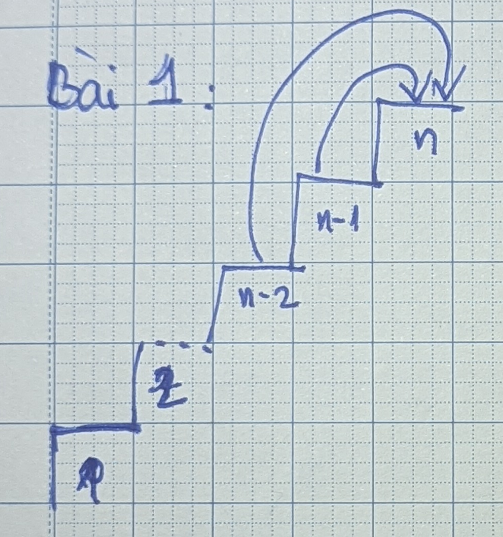
\includegraphics[width=0.3\textwidth]{image/Bai1.png}
\end{wrapfigure}

- Gọi \a{n} là số cách bước lên bậc thang thứ n. \\
- Do một lần có thể bước 1 hoặc 2 bước lên ta có 2 cách để bước lên bậc thang thứ $n$:
\begin{itemize}
    \item Từ bậc $n-1$.
    \item Từ bậc $n-2$.
\end{itemize}

- Với mỗi cách, ta lần lượt có \a{n-1} và \a{n-2} cách.\\
- Theo nguyên lý cộng, ta được:
$$
a_n = a_{n-1} + a_{n-2}
$$

- Để bước lên bậc thang thứ 1, ta có 1 cách $\Ra a_1 = 1$.\\
- Để bước lên bậc thang thứ 2, ta có 2 cách $\Ra a_2 = 2$.\\
- Mặt khác: $a_2 = a_0 + a_1 \Leftrightarrow a_0 = a_2 - a_1 = 2-1 = 1$.\\
- Sử dụng Maple để giải hệ thức đệ quy trên, ta được:
\begin{center}
\begin{verbatim}
f := rsolve({a(0) = 1, a(1) = 1, a(n) = a(n-1)+a(n-2)}, a(n)): simplify(f)
\end{verbatim}
\end{center}
$$
a_n = \left(\frac{1}{2} - \frac{\sqrt{5}}{10}\right)\left(\frac{-\sqrt{5}}{2} + \frac{1}{2}\right)^n + \left(\frac{1}{2} + \frac{\sqrt{5}}{10}\right)\left(\frac{\sqrt{5}}{2} + \frac{1}{2}\right)^n
$$

\subsection{Câu b}
\begin{wrapfigure}{R}{0.35\textwidth}
    \centering
    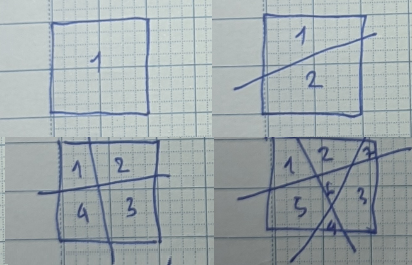
\includegraphics[width=0.35\textwidth]{image/Bai1b.png}
    \end{wrapfigure}
    
- Gọi \a{n} là số miền tối đa thu được khi chia mặt phẳng bằng $n$ đường thẳng.\\
- Nhìn vào các hình bên, ta thấy được: 
\begin{itemize}
    \item $a_0=1$
    \item $a_1=2$
    \item $a_2=3$
    \item $a_3=7$
    \item \dots 
\end{itemize}
.\\
Ta có thể thấy: $a_n = a_{n-1} + n$ với $a_0=1$.\\
Sử dụng Maple, ta thu được:
$$
a_n = \left(n+1\right)\left(\frac{1}{2}n+1\right)-n
$$

\subsection{Câu c}
\begin{figure}[H]
\centering
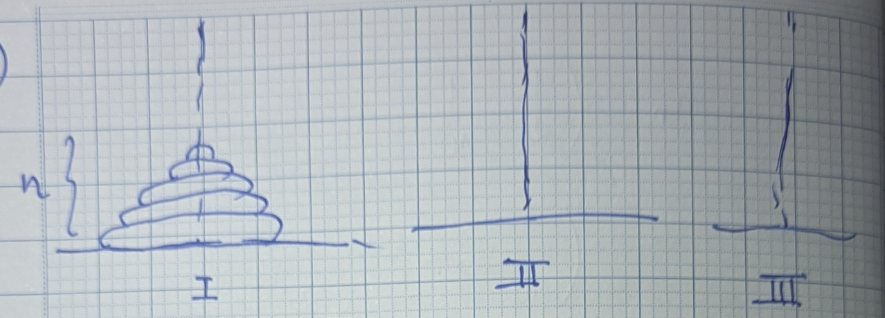
\includegraphics[width=0.6\textwidth]{image/Bai1c.png}
\end{figure}

- Gọi \a{n} là số cách di chuyển $n$ dĩa từ cột này sang cột khác. \\
- Giả sử, ta di chuyển $n$ dĩa này từ I sang II. Ta làm các bước sau:
\begin{itemize}
    \item Di chuyển $n-1$ dĩa từ I sang III:\\ Có \a{n-1} cách.
    \item Di chuyển dĩa lớn nhất từ I sang II:\\ Có 1 cách.
    \item Di chuyển $n-1$ dĩa khi nãy từ III sang II:\\ Có \a{n-1} cách.
\end{itemize}
- Theo nguyên lý cộng, ta có:
\begin{align*}
a_n &= a_{n-1} + 1 + a_{n-1} \\
 &= 2a_{n-1}+1 \\
\end{align*}
- \textbf{Tìm hệ số đầu:} khi ta di chuyển 1 dĩa thì có 1 cách nên \a{1} = 1.\\
- Mặt khác: $a_1 = 2a_0 + 1 \Leftrightarrow a_0 = {(a_1-1)}/{2}=0$.\\
- Sử dụng Maple, ta có:
$$
a_n = 2^n-1
$$
\end{document}